\chapter{Implementation Use Case:  Movie Booking}
\label{chap:movie}

\section{Overview}
In this chapter, we describe how Socrates Sim is adapted to support the movie domain. The goal of the movie booking agent is to help the end user purchase movie tickets. A similar dialog agent was developed for the \cite{li_usersim} paper. Unfortunately, we were unable to reuse their agent and domain knowledge base. Much of their data was crowdsourced from Amazon Mechanical Turk. There was a confusing overlap between the dialog action space for the user and agent, which resulted in the user simulator generating unrealistic utterances and dialog acts. There was also a high ratio of noise and data quality issues.  

Drawing inspiration from their use case, the agent we developed is simpler and modeled after something you would see on a site like Fandango. The agent will help identify movies for the user based on the user's preferences and also collect the user's payment details if the user chooses to book a ticket. As the goal for this implementation is mainly to demonstrate the end-to-end dialog simulation using a user simulator, we did not implement an actual reservation database, a payment processing system, and a large movie showtimes catalog. There are stubs for where the dialog agent would consult external resources while aiding the user. 

We focus below on the implementation details for the user simulator and domain modeling exercise. One of the primary benefits of Socrates Sim is that it can be retargeted to new domains. We do not need to reimplement the framework or dialog manager. We first define the new domain specific components (i.e., the dialog domain, user simulator, and dialog agent). Then we create a new simulation configuration file. Due to the modular nature of the Socrates Sim, we are also able to reuse much of the code developed for the restaurant domain. Most of the modules are written to be domain agnostic, and read in the domain-specific logic from external configuration files. This allows for rapid experimentation and code conservation.

\section{Defining Dialog Domain}

For the movie domain, we first set up the domain configuration file. This file is used to generate the domain object that will be used by both the user simulator and dialog agent. The inform and request slots reflect information that will be communicated and captured specifically for the movie book use case. For this use case, the user's preferences include movie genre, minimum movie rating, showtimes, and theater location. From the dialog agent's point of view, it will need to elicit the number of tickets the user wants to buy, the name of the movie, preferred showtimes, and theater location. Additionally, the agent will collect the user's credit card information to complete the "purchase" of the tickets. 

\begin{figure}[h!]
	\centering
	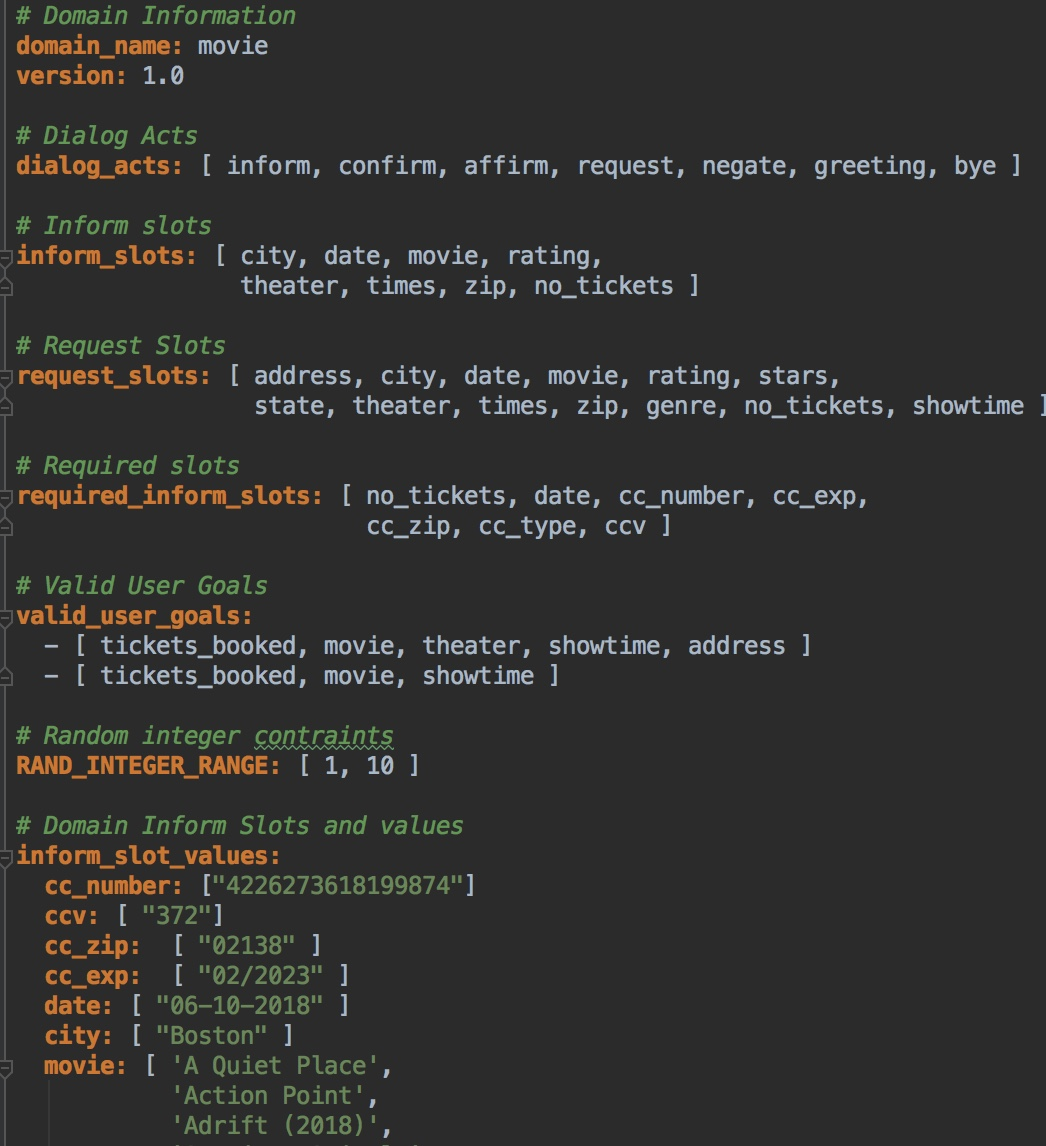
\includegraphics[scale=.25]{diagrams/movie_dialog_domain.jpeg}
	\caption{ Movie booking dialog domain configuration file. }
	\label{fig:movie_domain}
\end{figure}

The domain configuration file was designed to be flexible. Compared to the the configuration file for the restaurant domain, we introduce two new sections, \textit{required\_slots} and \textit{random\_integer\_range}. The required slots property indicates the inform slots that must be included in the user's goal. We require that the user goal include credit card information in the inform slots so that it can be presented to the dialog agent for "purchasing" tickets. The \textit{random\_integer\_range} is used to bound the range for generating a random positive integer. This random integer is used to indicate the number of tickets the user simulator wishes to purchase. 

The dialog configuration file is automatically converted into a domain object when Socrates Sim is loaded. Standard domain information (dialog acts, inform and request slots, valid goals) is mapped directly as object properties. Additional information is stored in a dictionary called \textit{additional\_params} in the domain object. This design allows the user flexibility in defining the domain while maintaining a minimum level of standardization. 

\subsection{Domain Knowledge Base}

The dialog agent uses a database of movie showtimes to lookup movie showings and makes movie recommendations. We generated a sample movie database by scraping Fandango movie data. Since the data is only meant to be a proof of concept, we limited scraping to a single location (movie theaters within 2 miles of Cambridge, MA) and showings for one week. We collected show times for about nine movies across six theaters offered and all possible showtimes. 

Unfortunately, Fandango does not make available genre information and star ratings about the movies on the website. We randomly assigned each unique movie genre from six genres (action, romance, comedy, adventure, thriller, and horror) and star rating score from 1 to 5. The scraped data was stored in a csv file. Like the restaurant domain, I created a \textit{DomainKBtable} class to provide a standard interface to query and sample data from the knowledge base. The knowledge base is represented as a pandas data frame in memory. 

\section{User Simulator Domain}

The underlying code and logic for the rule-based user simulator are similar to that of the user simulator used in the restaurant domain. We updated the goal space to support new goals relevant to the movie booking use case.

\begin{figure}[h!]
	\centering
	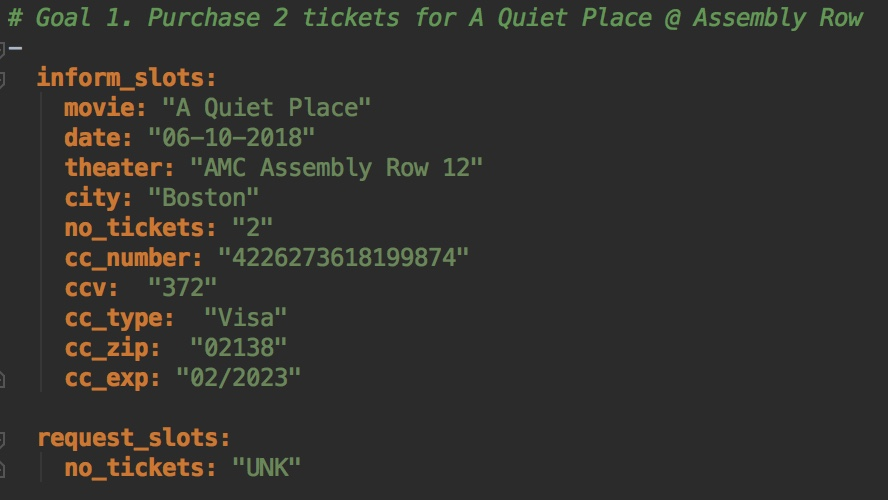
\includegraphics[scale=.25]{diagrams/sample_movie_goal.jpeg}
	\caption{ Example user goal for movie booking domain.}
	\label{fig:movie_goal}
\end{figure}

The internal logic for the user simulator is driven by a user agenda. For our implementation, we simply concatenate the inform and request slot lists stored in the user goal. For memory efficiency, we do not actually implement the agenda as an explicit stack. That information already exists in the user goal. Instead, we pop directly from the inform slots list in the user goal in response the dialog acts from the dialog agent. We keep track of the conversation state by checking how many of the request slots have been filled with real values. The rules-simulator runs sequentially through the request slots at the end of each conversation and updates its internal \textit{DialogStatus} enum object with one of two values: NO\_OUTCOME\_YET or FINISHED.

The logic for how the user simulator responds to incoming speech acts from the dialog agent is handled by the \textit{next} method. We reused the resolvers described in section \ref{sssec:logic}.

\begin{figure}[h!]
	\label{fig:movie_dispatch_tree}
	\begin{lstlisting}
 	self.response_router = {
 		"greetings": self._respond_general,
		"inform": self._respond_to_suggestion,
		"random_inform": self._respond_random_inform,
		"request": self._respond_request,
		"confirm": self._respond_confirm,
		"bye": self._respond_general
	}
	\end{lstlisting}
	\caption{ Internal dispatch tree for the movie booking user simulator.}
\end{figure}

The nlg and nlu processes are implemented as separate classes and described further in detail below. We can easily swap out implementations via the simulation configuration file, without having the modify the user simulator code directly.

\subsection{NLG and NLU}

For the movie domain, there were no publicly available datasets to seed a neural-based nlu model. We reused the \textit{NLUSimple} class from the restaurant domain. No new code had to be written. The rule-based model ingests a domain object and uses the domain's inform and request slot values for parsing. It should be noted that the rule-based nlu is brittle as it will use the literal slot values for reverse matching the entity. If the user simulator generates paraphrase or alters the spelling of the entity, the model will fail to map the entity to the appropriate slot type. For demonstration purposes, this is acceptable, as the goal of this use case is to demonstrate retargetability and flexibility of the framework.

We reused the \textit{UserSimNLGTemplate} class for natural language generation. Like \textit{NLUSimple}, the class is able to generalize to new domains by ingesting an external template file. We created a new nlg template file to support the various utterances that the user might say based on the combination of dialog act and dialog parameters. 

\begin{figure}[h!]
	\centering
	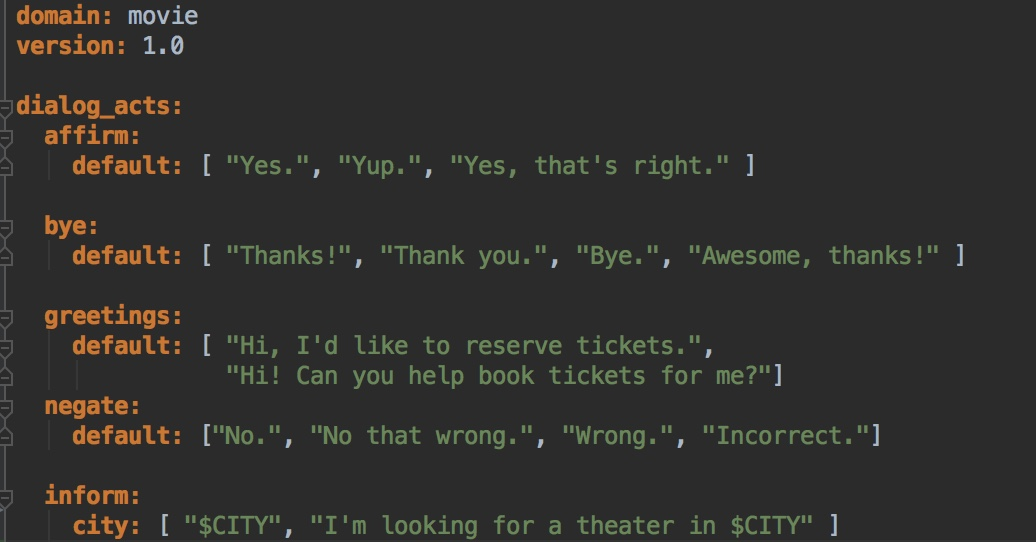
\includegraphics[scale=.25]{diagrams/movie_nlg_template.jpeg}
	\caption{Excerpt from nlg template for movie booking domain }
	\label{fig:movie_nlg}
\end{figure}

The key takeaway for this section is that no new code had to be written to support the nlu and nlg process for the movie booking user simulator. This demonstrates the value of creating a higher level NLU and NLG abstract base class. If the researcher wishes to build a more robust and finely tuned nlu and nlg models, they can easily plug it into the framework by extending the appropriate interface implementations of \textit{NLUSimple}/\textit{NLUModel} and the corresponding nlg classes. 

\section{Dialog Agent}

The movie booking agent was developed to illustrate how to incorporate an external dialog agent into the simulation framework. Since we do not have an existing movie booking agent, we developed a simple rule-based agent. The goal of the agent is to capture all the user's preferences and then make a suggestion from its knowledge base of Cambridge movie showings. Like the user simulator, the public facing methods the dialog manager interacts with are \textit{next} and \textit{get utterance}. 

For the movie booking agent, we follow a simple rules approach. The agent expects to interact with the following dialog acts: greetings, affirm, negate, request, inform, bye. In situations where the agent encounters an unknown dialog act, it will repeat its last dialog act. 

If the movie booking agent goes first, it issues a greetings action. If the agent is not responding to the user, it will then sequentially pop one item from it request slots and issue a request dialog act. Once the movie agent has collected information from the user, it will attempt to make a suggestion for movie showings from the knowledge base (\textit{DomainKBtable} object)  stored in the domain object. This is accomplished by calling the get suggestion method provided by the domain object. If the user accepts the suggestion. The dialog agent will then ask the user for information about their credit card details.

\section{Generating Sample Dialogs with Socrates Sim}

Once we have all the component pieces, we are able to run Socrates Sim. To run the simulations, we first created a simulation configuration file (Figure \ref{fig:movie_sim_config }). Socrates Sim dynamically loads the dialog domain, user simulator, and the dialog agent. As a result, changing from the restaurant domain to the movie domain just requires invoking Socrates Sim with a new configuration file. In the configuration file, we update the domain\_config, usersim\_class, and agent\_class to reflect the updated component locations. 

\begin{figure}[h!]
	\centering
	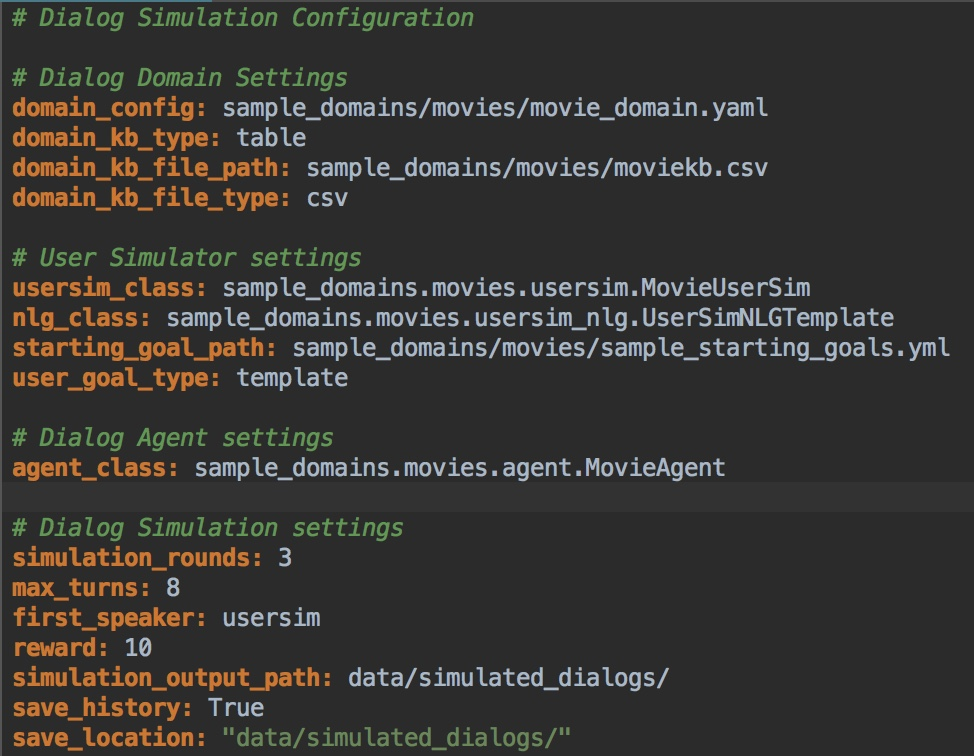
\includegraphics[scale=.3]{diagrams/movie_sim_config.jpeg}
	\caption{ Simulation configuration file. }
	\label{fig:movie_sim_config }
\end{figure}

\clearpage

Socrates Sim is invoked using the command-line and expects the path to the configuration file as an input. The figure below shows some example output for the sample dialogs that were generated by the simulator.

\begin{figure}[h!]
	\centering
	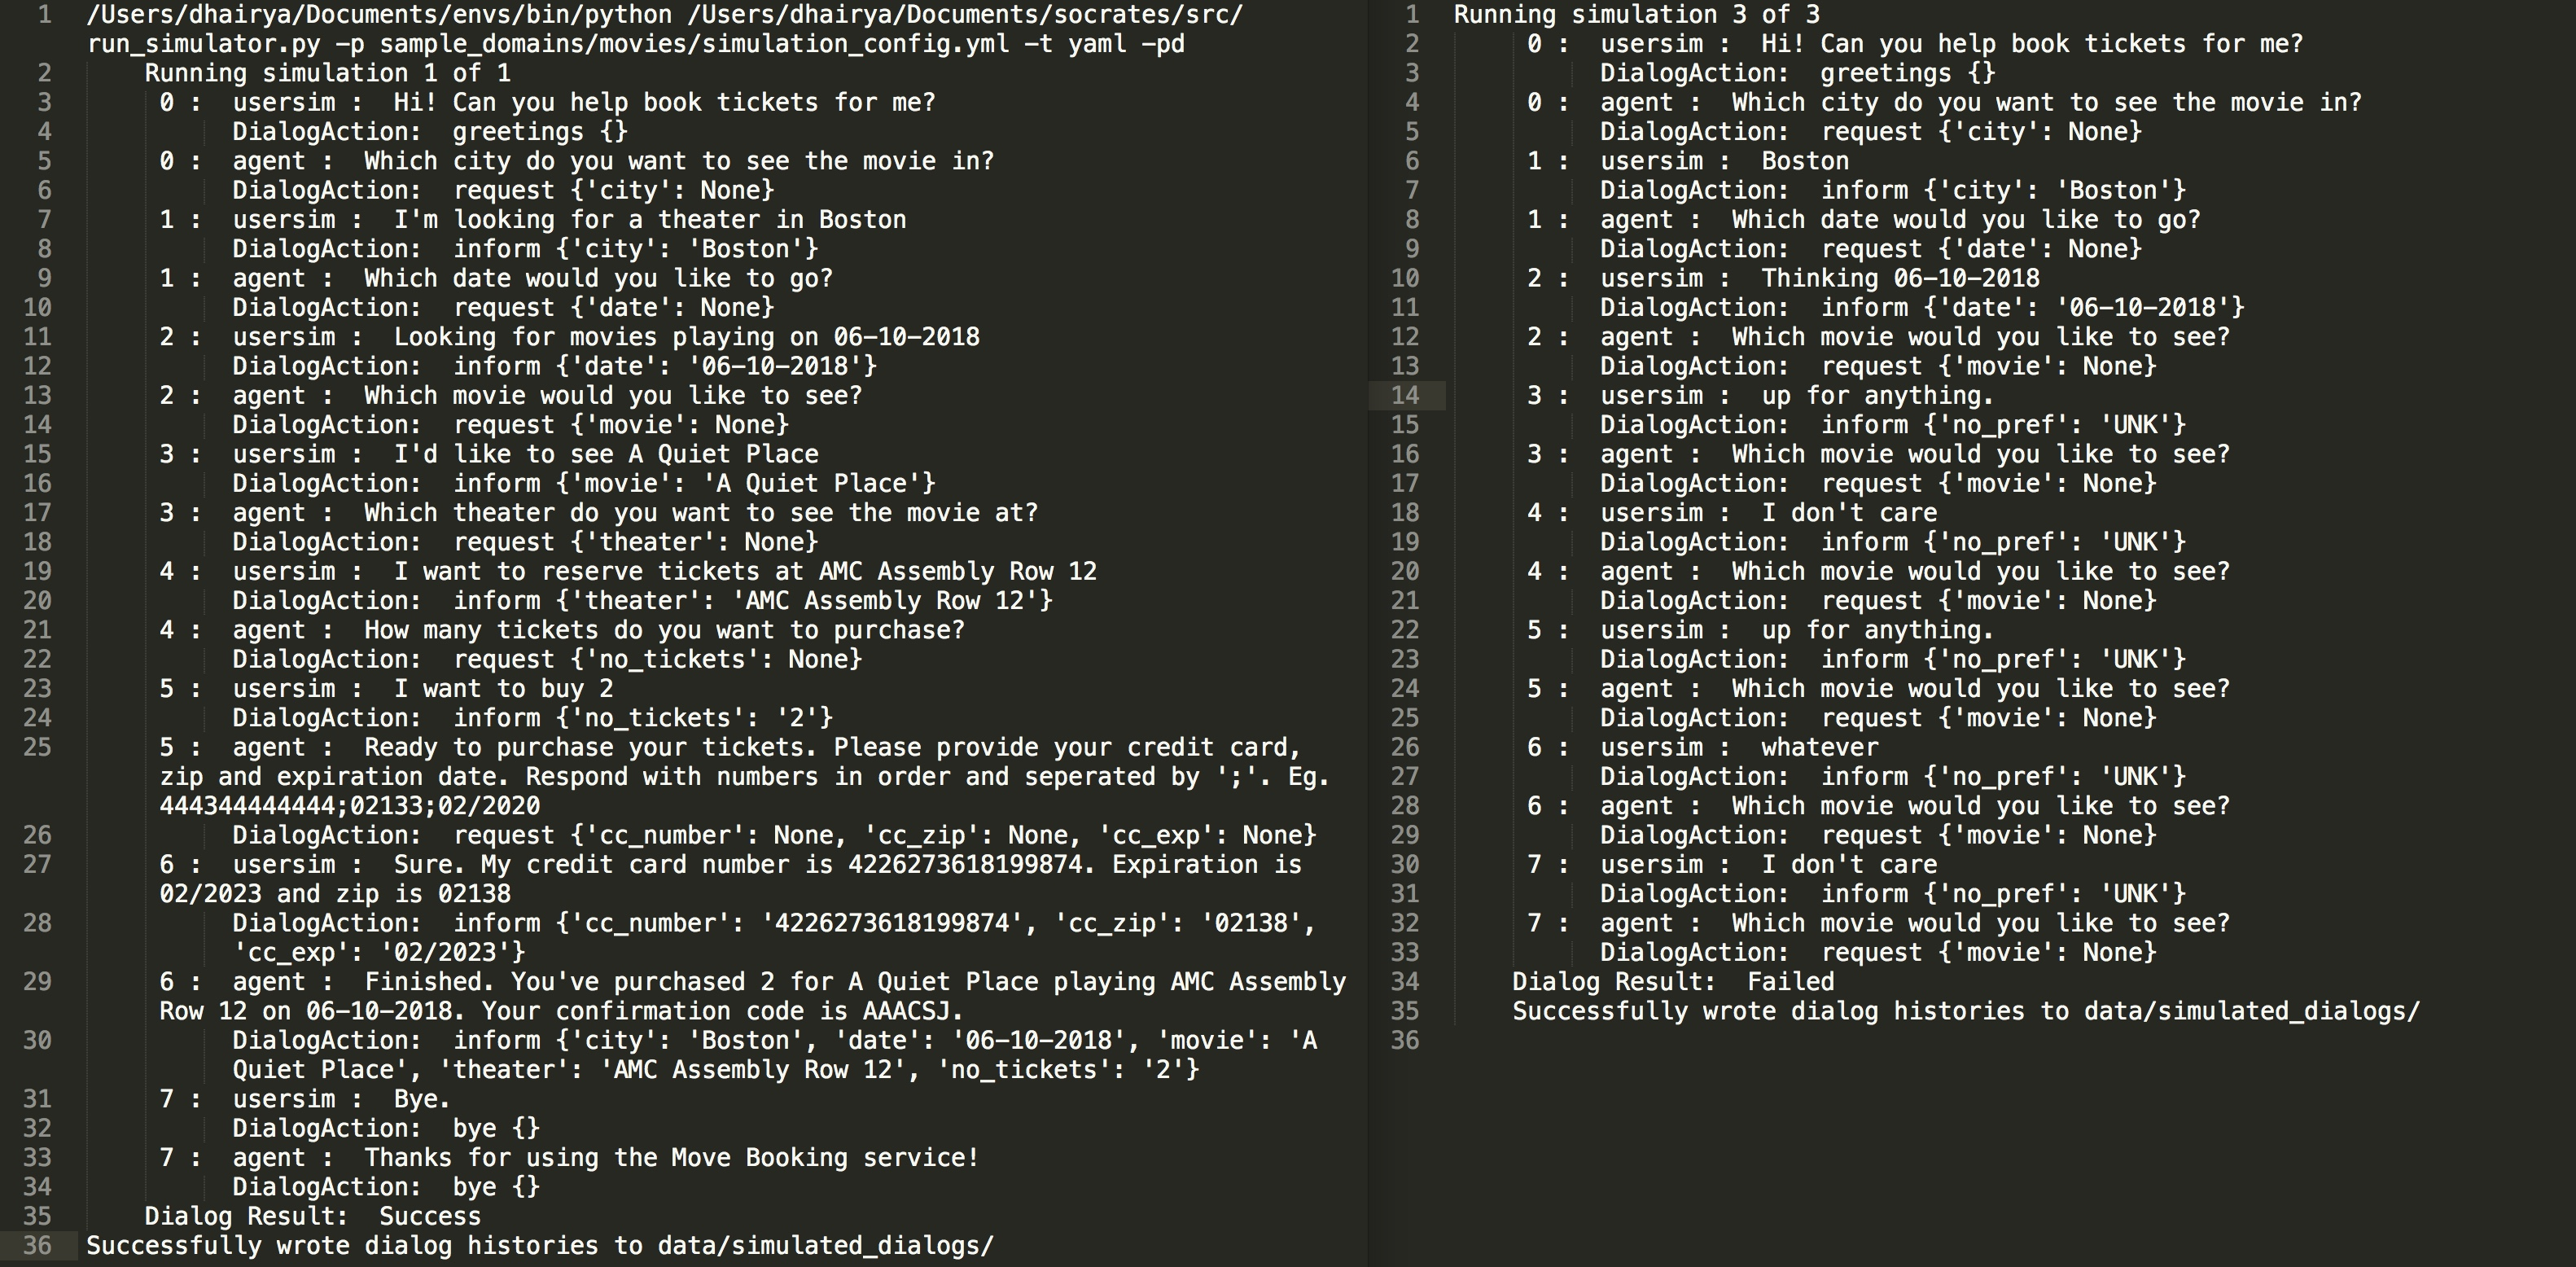
\includegraphics[scale=.15]{diagrams/movie_output.jpeg}
	\caption{ Sample dialog generated by Socrates Sim.}
	\label{fig:movie_output}
\end{figure}




%%% Local Variables: 
%%% mode: latex
%%% TeX-master: "main"
%%% End: 